\documentclass[fleqn,12pt,a4paper,twoside]{article}

\usepackage{graphicx,calc,soul,amsmath,fancyhdr,psfrag,tikz}
\usepackage{enumitem}
\usepackage{listings}
\usetikzlibrary{shapes.geometric,arrows}

% Set the dimensions of the paper.
\setlength{\paperwidth}{210mm}
\setlength{\paperheight}{297mm}

% Set the dimensions of the text.
\setlength{\textwidth}{\paperwidth-6cm}
\setlength{\textheight}{\paperheight-2in}

\setlength{\headheight}{15pt}
\setlength{\marginparwidth}{3cm - \marginparsep -0.25in}

% Adjust margins to fit the paper and text dimensions.
\setlength{\oddsidemargin}{0.5\paperwidth-0.5\textwidth-1in}
\setlength{\evensidemargin}{\oddsidemargin}
\setlength{\topmargin}{0.5\paperheight-0.5\textheight-1in-\headheight-\headsep}

\markright{Experiment 3F1: Flight Control}

\begin{document}
\thispagestyle{empty}

\begin{center}
\bfseries
\rule{\textwidth}{.8mm} \\[.3cm]
ENGINEERING TRIPOS PART IIA\\[1.5cm]
ELECTRICAL AND INFORMATION ENGINEERING\\
TEACHING LABORATORY\\[1.5cm]
MODULE EXPERIMENT 3F1 \\[1.5cm]
FLIGHT CONTROL\\
\rule{\textwidth}{.8mm}\\[.5cm] 
\end{center}
\vfill
\subsection*{Objectives:}

\begin{itemize}
\item Simulation of various aircraft models on the computer.
\item Study real-time (manual) control and the limitations imposed
by time delays.
\item Design of a simple autopilot.
\item Illustrate frequency response concepts in analogue and digital control 
systems, conditions for oscillation in feedback systems and stability.
\item Gain familiarity with Python and Jupyter Notebooks.
\end{itemize}
\vfill\vfill\null

\newpage
\thispagestyle{empty}
\null
\vfill
\begin{center}
\bfseries \mbox{}
%This page has intentionally been left blank.
\end{center}
\vfill
\null
\newpage

\section*{Getting Started}

\begin{itemize}[itemsep=-2pt]
        \item Log on to the teaching system. The computers in the EIETL should already be configured to log in to the Linux side of the teaching system, do not log in to the Windows side.
        \item Under \texttt{Activities}, select \texttt{Start 3F1 Flight Control}. This will create a \texttt{3F1\_Flight\_Control} directory in your home directory, and you will be able to access its contents later from any computer on the teaching system.
        \item Once the files are copied over, a Jupyter Notebook will launch automatically. All further instructions for the lab, including how to complete the worksheet, how to write your report, and how to submit your work, are contained within the notebook.
        \item The worksheet and report template are located at the end of this document.
\end{itemize}
\vspace*{-2.0em}
\subsubsection*{Troubleshooting}

If the Jupyter notebook does not launch from the \texttt{Start 3F1 Flight Control} shortcut, you can run it manually from within the \texttt{3F1\_Flight\_Control} directory via the following terminal commands:
\begin{lstlisting}[language=sh]
source /usr/local/python-venv/bin/activate
jupyter notebook 3f1_lab.ipynb
\end{lstlisting}
\hrulefill
\vspace*{-1.5em}
\section*{Instructions for a Full Technical Report}

Students not intending to submit a Full Technical Report on the 3F1 Lab may ignore this section. Guidance on the preparation of FTRs is provided in the CUED booklet \emph{A Guide to Report Writing}, with which you were issued in the first year.
If you are offering a FTR on this experiment, you should include a discussion section with seven subsections addressing the following points. Include your Laboratory Report as an appendix and refer to it where appropriate.

\subsubsection*{[1] The Stabilisation of Sinusoidal Disturbances}

\textbf{From §2.4:} Use the results of your calculations
to indicate $K(j\omega_1)G(j\omega_1)$, where $\omega_1=0.66 \times
2 \pi$ rad/s, on an Argand diagram for suitable stabilising
proportional gains and hence estimate $| (1 +
K(j\omega_1)G(j\omega_1))|$. Does the theory predict that your
feedback will help attenuate the sinusoidal disturbance for
stabilizing gains?  How does this compare to your experience given in your lab report?

\subsubsection*{[2] Unstable Aircraft}

\textbf{From §2.5:} It turns out that if $D > T$ then no
proportional gain exists to stabilise the system. Verify this claim
analytically in your report.

\subsubsection*{[3] Broom Balancing}

The problem of stabilizing an unstable aircraft is similar in many
respects to the problem of balancing a broom.

Consider the question: ``What is the shortest upside down broom I can
balance on my hand?'' The linearised equations of motion (assuming
negligible handle weight, length $L$, horizontal position of your hand
$x$, angle $\theta$ to vertical, and considering one dimension) are:
\begin{equation}
        \ddot{x} + L\ddot{\theta} = g\theta \nonumber
\end{equation}
Suppose we measure the horizontal position of the top of the broom,
$y=x+L\theta$ and then use the feedback signal, $z=y+T\dot{y}$
where $T^2 = L/g$.  Calculate the transfer function from $x$ to $z$
under this arrangement.

This assumes the particular proportional-derivative action controller
given, but this is a reasonable choice.  Do you notice a similarity
with the dynamics of the unstable aircraft?

Hence provide estimates of the minimum value of $L$ based on
your above results. Compare this with reality, and comment.

\subsubsection*{[4] PID Derivative Term Approximation}

\textbf{From §3.3:} Review the code implementing the PID Controller. Which method was used to approximate the
derivative? Calculate the transfer function of
the discretised controller ($z$-domain) assuming that the simulation runs at a consistent 60 frames per second.

\subsubsection*{[5] Discretised Time Delays}

Consider the discretisation of blocks with time-delays. Consider the continuous time plant $G(s)=e^{-D_1s}/s$ placed in the
arrangement illustrated in Figure~\ref{adc}.  Find the discrete-time
transfer function from $u(k)$ to $y(k)$.  The DAC is a simple zero
order hold, and you may assume that the ADC and DAC operate
synchronously with sampling period $T$ (Hint: You may find it useful
to write $D_1=nT+D_0$ where $n$ is an integer and $0\leq D_0<T$).

\begin{figure}[htb]
        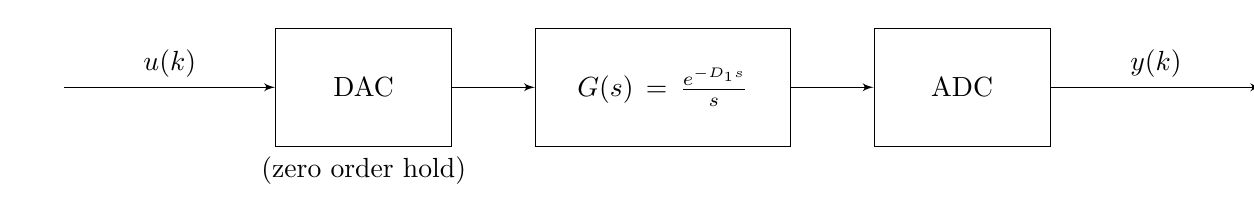
\begin{tikzpicture}[auto, node distance=3.8cm, >=latex']
                % Define block styles
                \tikzstyle{input} = [coordinate]
                \tikzstyle{output} = [coordinate]
                \tikzstyle{block} = [draw, rectangle, text width=2cm, text centered, minimum height=1.5cm]
            
                % Define blocks
                \node [input, name=input] (input) {};
                \node [block, right of=input] (dac) {DAC};
                \node [block, text width=3cm, right of=dac] (transfer) {$G(s)=\frac{e^{-D_1 s}}{s}$};
                \node [block, right of=transfer] (adc) {ADC};
                \node [output, right of=adc] (output) {};
            
                % Connect blocks
                \draw [->] (input) -- node {$u(k)$} (dac);
                \draw [->] (dac) -- node {} (transfer);
                \draw [->] (transfer) -- node {} (adc);
                \draw [->] (adc) -- node {$y(k)$} (output);
        
                \node [below] at (dac.south) {(zero order hold)};
            \end{tikzpicture}
       \caption{ADC/DAC arrangement for discretization}
        \label{adc}
\end{figure} 

The plotting functions for producing Bode diagrams used by the lab obtains a time-delayed frequency response for the continuous system by first calculating the frequency response of the plant and then shifting it by a time delay corresponding to $e^{-Ds}$. However, the simulation runs in discrete time, and treats input as a zero-order hold. Discuss any changes in accuracy that might arise from using this scheme with a low sampling rate.

\subsubsection*{[6] Discrete Systems}

Complete \textbf{§4: Discrete Systems} in the lab notebook, including answers to the questions and requested figures.

\pagebreak

\thispagestyle{empty}
\section*{3F1 Lab Worksheet}

\begin{tabbing}
\textbf{2.1 Simplified Aircraft Model} \\[3mm]
Transfer function $=$ \\[3mm]
\verb+num =+ \hspace*{2cm} \verb+den =+\\
\end{tabbing}

\begin{tabbing}
        \textbf{2.2 Modelling Manual Control}\\[3mm]
        Controller transfer function $=$\\[3mm]
$k=$ \hspace*{2cm} $D=$\\[3mm]

Phase margin $=$\\[3mm]

Amount of extra time delay which can be tolerated $=$\\
\end{tabbing}

\begin{tabbing}
\textbf{2.3 Pilot Induced Oscillation}\\[3mm]

Period of oscillation (observed) $=$\\[3mm]

Period of oscillation (theoretical) $=$\\
\end{tabbing}

\begin{tabbing}
\textbf{2.4 Sinusoidal disturbances}\\[3mm]
\= Maximum stabilising gain $=$\\[3mm]
                \> Gain at 0.66 Hz $=$ \hspace*{4cm} \= Phase at 0.66 Hz $=$\\[1mm]
\end{tabbing}

\begin{tabbing}
        \textbf{2.5 Unstable Aircraft}\\[3mm]
        Fastest pole at $T=$\\[3mm]
\end{tabbing}

\begin{tabbing}
\textbf{3.2 Autopilot with Proportional Control}\\[3mm]
\= Proportional gain $K_c=$ \hspace*{2cm} Period of oscillation $T_c=$\\
\end{tabbing}

\begin{tabbing}
\textbf{3.3 Autopilot with PID Control}\\[3mm]
Transfer function of PID controller $=$\\[3mm]
PID constants: $K_p = \hspace*{1.5cm} T_i = \hspace*{1.5cm} T_d = \hspace*{1cm}$\\[4mm]
Adjusted value of \,$T_d = $\\
\end{tabbing}

\begin{tabbing}
\textbf{3.4 Integrator Wind-up}\\[3mm]
Integrator bound $Q=$\\
\end{tabbing}

\pagebreak

\newpage
\thispagestyle{empty}
\null
\vfill
\begin{center}
\bfseries \mbox{}
%This page has intentionally been left blank.
\end{center}
\vfill
\null
\newpage

\section*{Report Template (3F1 Flight Control Lab)}

This report template contains \textbf{9 questions} spread over \textbf{4 pages}.

\vspace{2cm}

\noindent \textbf{1.} (§2.2 Modelling Manual Control) Nyquist diagram (from Bode diagram) for controller in series with plant.

\begin{center}
\begin{tikzpicture}[scale=1.3]
        \draw[->] (3,0) -- (9,0) node[right] {Re};
        \draw[->] (6,-3) -- (6,3) node[above] {Im};
        \node[align=center,font=\footnotesize] at (6,-3.5) {Nyquist diagram};
\end{tikzpicture}
\end{center}

\noindent \textbf{2.} (§2.2 Modelling Manual Control) Are you using any integral action? Give a brief explanation. What does this imply about the accuracy of the model of the human controller?

\vspace{8cm}

\pagebreak

\noindent \textbf{3.} (§2.3 Pilot Induced Oscillation) Explain the oscillation of the feedback loop.
How does your observed period of oscillation compare to the theoretical prediction?

\vspace{5cm}

\noindent \textbf{4.} (§2.3 Pilot Induced Oscillation) Can you give a rough guideline to the control designer to make PIO less likely?

\vspace{5cm}

\noindent \textbf{5.} (§2.4 Sinusoidal Disturbances) Was your manual input able to reduce the error (as compared to providing no input)?

\vspace{5cm}
\pagebreak

\noindent \textbf{6.} (§2.5 An Unstable Aircraft) Nyquist diagram for $G_2(s).$
\begin{center}
\begin{tikzpicture}[scale=1.3]
        \draw[->] (-2,0) -- (2,0) node[right] {Re};
        \draw[->] (0,-2) -- (0,2) node[above] {Im};
        \node[align=center,font=\footnotesize] at (0,-2.5) {Nyquist diagram of $G_2(s)$};
\end{tikzpicture}
\end{center}

\noindent \textbf{7.} (§2.5 An Unstable Aircraft) Explain, using the Nyquist criterion, why the feedback system is stable with a proportional gain greater than 0.5.

\vspace{5cm}

\noindent \textbf{8.} (§2.5 An Unstable Aircraft) Sketch of a Nyquist diagram for $G_2(s).$ with a small time delay $D$.
\begin{center}
        \begin{tikzpicture}[scale=1.3]
                \draw[->] (-2,0) -- (2,0) node[right] {Re};
                \draw[->] (0,-2) -- (0,2) node[above] {Im};
                \node[align=center,font=\footnotesize] at (0,-2.5) {Nyquist diagram with small time delay};
        \end{tikzpicture}
\end{center}

\pagebreak

\noindent \textbf{9.} (§3.4 Integrator Wind-up) Explain how you calculated the bound on $Q$.


\end{document}
